\documentclass[tikz,border=8pt]{standalone}
\usepackage{tikz}
\usetikzlibrary{arrows.meta,positioning}
\begin{document}
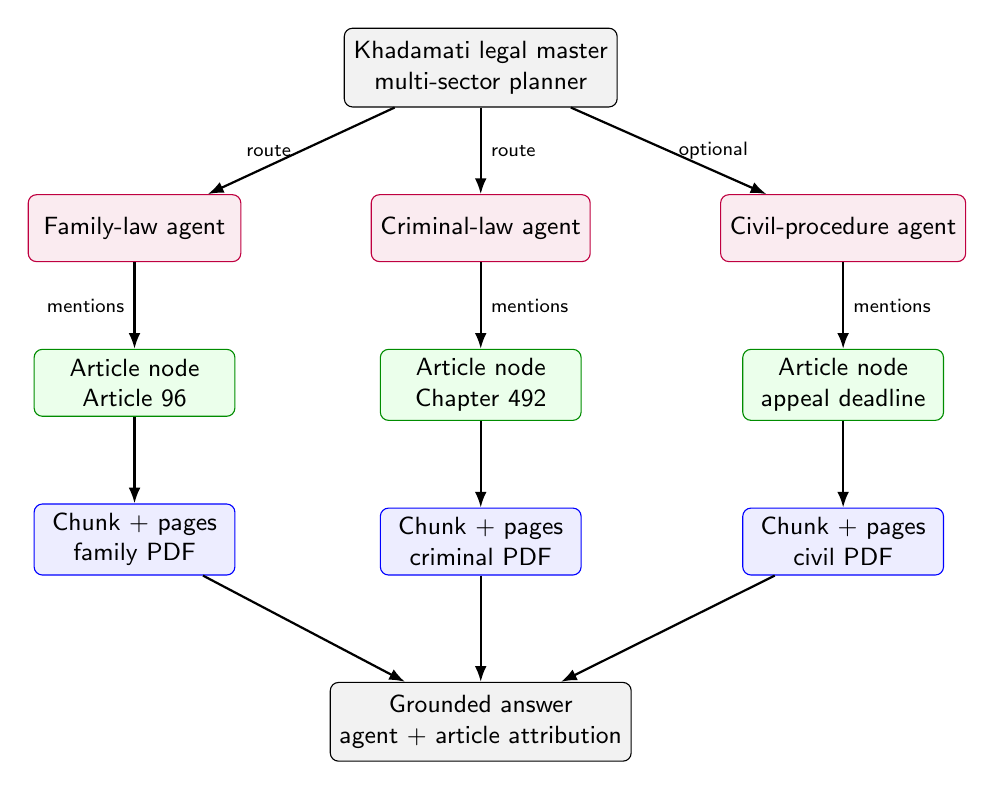
\begin{tikzpicture}[
  node distance=1.1cm and 1.3cm,
  hub/.style={draw=black, fill=black!5, rounded corners=3pt, align=center, minimum width=3.2cm, minimum height=1cm, font=\sffamily\small},
  agent/.style={draw=purple, fill=purple!8, rounded corners=3pt, align=center, minimum width=2.7cm, minimum height=0.85cm, font=\sffamily\small},
  article/.style={draw=green!55!black, fill=green!8, rounded corners=3pt, align=center, minimum width=2.55cm, minimum height=0.85cm, font=\sffamily\small},
  chunk/.style={draw=blue, fill=blue!7, rounded corners=3pt, align=center, minimum width=2.55cm, minimum height=0.85cm, font=\sffamily\small},
  arrow/.style={-{Latex[length=2mm]}, line width=0.8pt}
]
  \node[hub] (master) {Khadamati legal master\\multi-sector planner};

  \node[agent, below left=of master] (family) {Family-law agent};
  \node[agent, below=of master] (criminal) {Criminal-law agent};
  \node[agent, below right=of master] (civil) {Civil-procedure agent};

  \node[article, below=of family] (a1) {Article node\\Article 96};
  \node[article, below=of criminal] (a2) {Article node\\Chapter 492};
  \node[article, below=of civil] (a3) {Article node\\appeal deadline};

  \node[chunk, below=of a1] (c1) {Chunk + pages\\family PDF};
  \node[chunk, below=of a2] (c2) {Chunk + pages\\criminal PDF};
  \node[chunk, below=of a3] (c3) {Chunk + pages\\civil PDF};

  \node[hub, below=1.35cm of c2] (answer) {Grounded answer\\agent + article attribution};

  \draw[arrow] (master) -- node[left, font=\sffamily\scriptsize]{route} (family);
  \draw[arrow] (master) -- node[right, font=\sffamily\scriptsize]{route} (criminal);
  \draw[arrow] (master) -- node[right, font=\sffamily\scriptsize]{optional} (civil);
  \draw[arrow] (family) -- node[left, font=\sffamily\scriptsize]{mentions} (a1);
  \draw[arrow] (criminal) -- node[right, font=\sffamily\scriptsize]{mentions} (a2);
  \draw[arrow] (civil) -- node[right, font=\sffamily\scriptsize]{mentions} (a3);
  \draw[arrow] (a1) -- (c1);
  \draw[arrow] (a2) -- (c2);
  \draw[arrow] (a3) -- (c3);
  \draw[arrow] (c1) -- (answer);
  \draw[arrow] (c2) -- (answer);
  \draw[arrow] (c3) -- (answer);
\end{tikzpicture}
\end{document}
